% One-dimensional data
\subsection{One Dimension}
\subsubsection{Simple Reward Function}
As a very basic proof of concept, we ran the algorithms on the reward
function $r(x) = x$ over the unit interval [0,1].

\begin{figure}[!ht]
  \begin{center}
    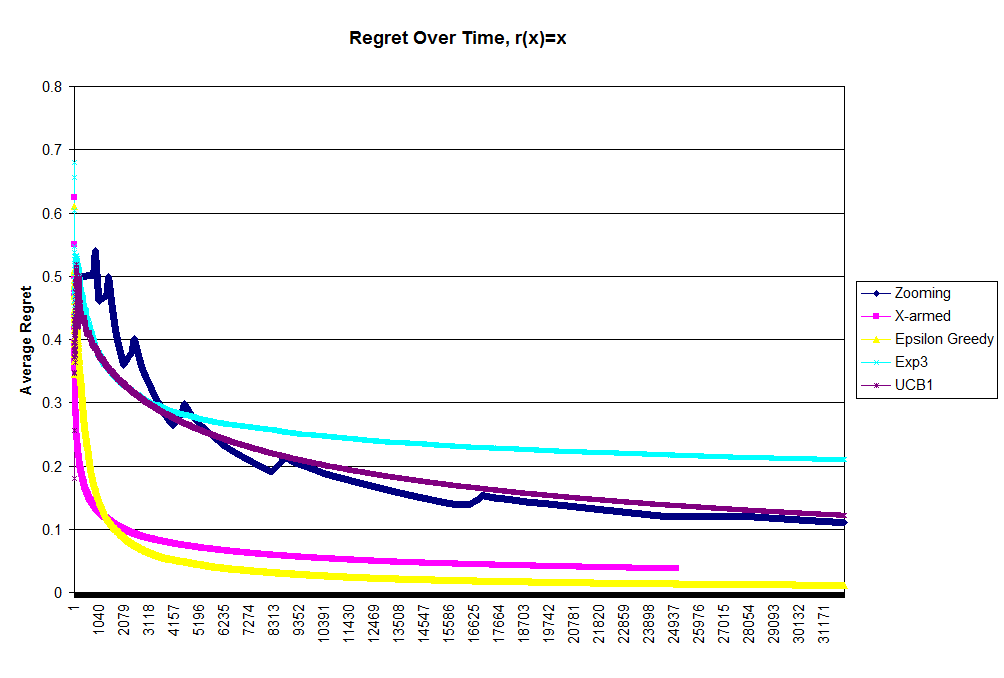
\includegraphics[width=\figwidth]{figures/1dsimpleplot.png}
     \caption{$r(x) = x$, 100 arms for discretization
     algorithms}
     \label{fig:1dsimple}
  \end{center}
\end{figure}

From figure \ref{fig:1dsimple}, we can see a number of facts.  First, at 
least in this case, the $\epsilon$-greedy algorithm is clearly the
best of all discretization algorithms, which is due to there being
no noise.  The $\mathcal{X}$-armed algorithm also does rather well,
but becomes expensive computationally as the number of rounds becomes
large due to having $O(n)$ time complexity in each round, where $t$ is
the number of rounds so far.  We can also see the characteristic bumps of
the Zooming algorithm, which are indicative of the fact that the Zooming
algorithm does not carry over information between phases.


\subsubsection{Noisy Reward Function}
Now we shall add some noise to our reward function.  The new reward
function is $r(x) = b(n_{0,1}(x))$, where $b(x) = 1$ with probability
$x$ and is 0 otherwise and $n_{\alpha_,\beta}(x)$ is $x$ times a random
number uniformly drawn from the interval $[\alpha, \beta]$.  The results
are presented in figure \ref{fig:1dnoise}

\begin{figure}[!ht]
  \begin{center}
    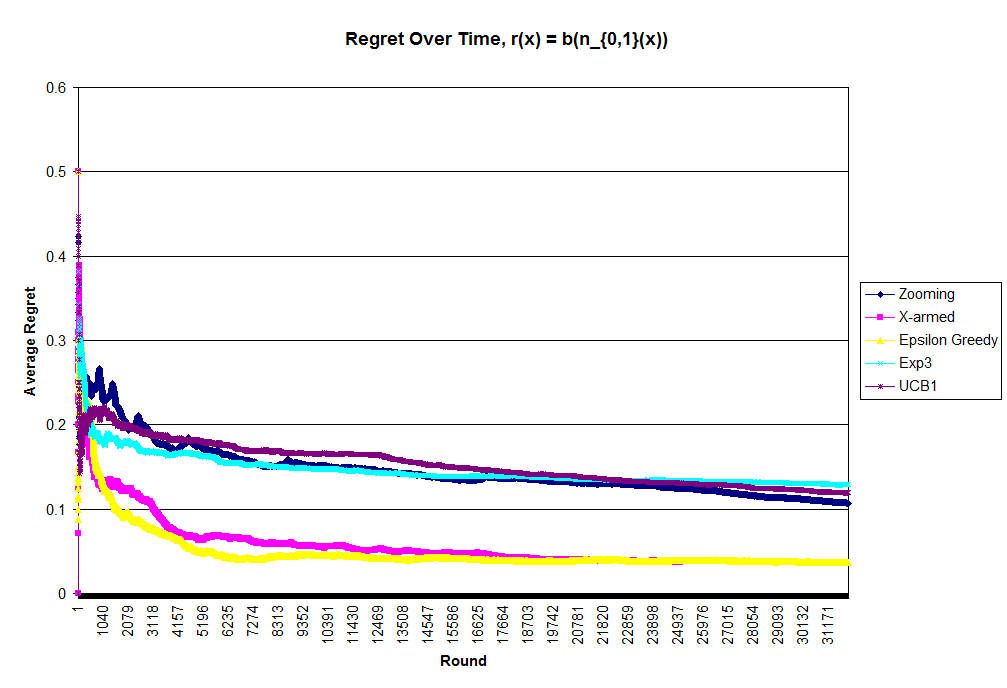
\includegraphics[width=\figwidth]{figures/1dnoiseplot.png}
     \caption{$r(x) = b(n_{0,1}(x))$, 100 arms for discretization
     algorithms}
     \label{fig:1dnoise}
  \end{center}
\end{figure}

For the most part, the algorithms perform basically as well as they did
in the no-noise case, with the notable exceptions that Exp3 algorithm did
better than before and the $\epsilon$-greedy algorithm did slightly worse
than before.  In the case of the $\epsilon$-greedy algorithm, this can be
partially attributed to the fact that the random discretization determines
how low the average regret can get, and that in this particular trial
the discretization was not very good.  We can tell that this is the true
reason for this behavior because otherwise, the $\epsilon$-greedy algorithm
would be converging more slowly, which does not appear to be the case.

Overall, from these simple 1D cases, we can see that
$\mathcal{X}$-armed algorithm appears to perform better than the Zooming
algorithm, although at the cost of being rather slow when the number of
rounds becomes large.  In a bandit setting, though, it is generally the
case that the reward function is somewhat costly to evaluate, and so the
computational cost of the $\mathcal{X}$-armed algorithm is not quite so
important.  Also, if we look at the very first few trials, the
$\mathcal{X}$-armed algorithm does fairly well rather quickly, whereas
the other algorithms take a little bit longer to fully explore the space.
For the discretization algorithms, though, this can be mitigated by
choosing a smaller number of arms to discretize the domain into.  In fact,
the very number of arms chosen for those algorithms is essentially a 
parameter helping to determine how much exploration to do -- more arms
will cause more exploration, and fewer arms will cause more exploitation.